% Copyright 2026 Sreeram Anil
% SPDX-License-Identifier: CC-BY-4.0
% =============================================================================
%  Online ELM residual learner inside an EKF (ELM-RLS-EKF)
% =============================================================================
\chapter{Online extreme-learning-machine residual EKF (ELM-RLS-EKF)}
\label{ch:elmrlsekf}

\section*{At a glance}
\begin{tabular}{@{}l>{\raggedright\arraybackslash}p{0.76\textwidth}@{}}
Family & learning (data-driven) \\
Header & \texttt{include/estkit/learning/elm\_rls\_ekf.hpp} \\
Registered name & \texttt{ELM-RLS-EKF} \\
State dimension & $n_x = 4$; $n_\varphi = n_h + n_\xi = 26$ learned weights \\
Cost per step & EKF $\mathcal{O}(n_x^3)$ plus RLS $\mathcal{O}(n_\varphi^2)$;
measured \SI{3.3}{\micro\second}, no heap \\
Memory & \SI{11.4}{\kilo\byte} (the $26\times26$ RLS covariance dominates) \\
Primary references & \cite{huang2006elm,liang2006oselm,pao1994rvfl,ljung1999,friedland1969bias} \\
\end{tabular}

\section{Motivation and aerospace/BMS relevance}
The hybrid of Chapter~\ref{ch:nnekf} buys accuracy on the cells it was characterised against and
pays for it on every other cell.  The natural next question is whether the residual can be learned
\emph{during the flight}, from the filter's own innovation sequence, so that no characterisation
campaign, no frozen weight table and no operational-design-domain argument is needed.  A battery
pack in service drifts continuously --- resistance grows with age, contact resistance grows with
vibration cycles, a cold-soaked pack behaves differently from a heat-soaked one --- and a residual
model that adapts is exactly what a maintenance-free system wants.

Two ingredients make online learning tractable in a \SI{10}{\hertz} embedded task.  The first is
the extreme learning machine \citep{huang2006elm}: draw the hidden layer's weights \emph{once} from
a fixed pseudo-random stream and never touch them again, so that only the output layer remains to
be identified --- and that is a \emph{linear} least-squares problem, solvable recursively
\citep{liang2006oselm} at $\mathcal{O}(n_\varphi^2)$ per sample with no gradients and no
backpropagation.  The second is the direct linear link of the random vector functional-link net
\citep{pao1994rvfl}: appending the raw regressor to the random features guarantees that the
physically dominant residual of a resistance error, $-\Delta R_0\, i$, is represented
\emph{exactly} rather than approximated by whatever \texttt{tanh} ridges the random draw happened
to produce.

There is, however, a catch that no amount of engineering removes and that this chapter treats as
its main subject: \textbf{an output-bias model and a state-of-charge error are locally
indistinguishable}.  Left unconstrained, the residual learner will absorb the SOC error, the
corrected innovation will go to zero, the filter will stop correcting, and the estimate will decay
into open-loop Coulomb counting while every internal consistency check still passes.  This is not
a hypothetical: it is what the first implementation of this estimator actually did, and
Section~\ref{sec:elm-ident} shows the measured trace.

\section{Problem statement and assumptions}
The plant is the ECM of Chapter~\ref{ch:ecm} with an unknown, slowly varying output disturbance:
\begin{equation}\label{eq:elm-plant}
\vx_{k+1} = f(\vx_k,\vu_k) + \vw_k,\qquad
y_k = h(\vx_k,\vu_k) + \rho_k + \vv_k,
\end{equation}
where $\rho_k\in\real$ is the unmodelled output term.  The method assumes:

\begin{assumption}[Exogenous structure]\label{as:elm-exo}
$\rho_k$ is well approximated by a static function of the \emph{inputs} $\vu_k = [i_k, T_k]^\T$
alone: $\rho_k \approx \rho(\vu_k)$.
\end{assumption}

\begin{assumption}[Time-scale separation]\label{as:elm-ts}
$\rho(\cdot)$ varies slowly compared with the excitation of $\vu_k$, so that the input variation
within the RLS memory $1/(1-\lambda)$ identifies it.
\end{assumption}

\begin{assumption}[Persistent excitation]\label{as:elm-pe}
The current profile excites the regressor: $\frac{1}{N}\sum_k \varphi_k\varphi_k^\T \succ 0$ over
any window of length $1/(1-\lambda)$.
\end{assumption}

Assumption~\ref{as:elm-exo} is a deliberate restriction, and Section~\ref{sec:elm-ident} explains
why it, rather than the more permissive $\rho(\soc,i,T)$ of the original proposal, is the version
that works.  Assumption~\ref{as:elm-pe} is satisfied by a real flight profile, where the current
swings between $0.2$ and $4.5$ times the $1$-hour rate, and violated by a constant-current
bench test --- where, correctly, nothing is identifiable.

\section{Derivation}

\subsection{Random feature map}
The regressor is assembled from the model input and, optionally, the state, each centred and scaled
so that the random layer operates in its non-saturated range:
\begin{equation}\label{eq:elm-xi}
\xi_k = \begin{bmatrix} (\vu_k - \vu_c)\odot \vu_s \\[2pt]
                        m_x \odot (\xminus_k - \vx_c)\odot \vx_s \end{bmatrix}\in\real^{n_\xi},
\qquad n_\xi = n_u + n_x = 6,
\end{equation}
with the mask $m_x = 0$ unless \texttt{use\_state\_features} is set.  For the cell model
$\vu_c = [0, T_0]^\T$ and $\vu_s = [1/8, 1/15]^\T$ (current in \si{\ampere}, temperature in
\si{\kelvin}).  The feature vector combines $n_h = 20$ random \texttt{tanh} ridges with the direct
linear link \citep{pao1994rvfl}:
\begin{equation}\label{eq:elm-phi}
\varphi_k = \bigl[\ \tanh(a_1^\T\xi_k + b_1),\ \dots,\ \tanh(a_{n_h}^\T\xi_k + b_{n_h}),\ \xi_k^\T\ \bigr]^\T
\in\real^{n_\varphi},\quad n_\varphi = n_h + n_\xi = 26,
\end{equation}
with $a_m\sim\mathcal{U}(-\num{1.5},\num{1.5})^{n_\xi}$ and $b_m\sim\mathcal{U}(-1,1)$ drawn once
from the deterministic \texttt{xoshiro256**} stream \citep{blackman2021xoshiro} and \emph{frozen}:
the hidden layer is part of the delivered artefact, not a run-time random variable.  The learned
residual is
\begin{equation}\label{eq:elm-rho}
\hat\rho_k = \operatorname{sat}_{r_{\max}}\!\bigl(\vtheta_k^\T\tilde\varphi_k\bigr),
\qquad r_{\max} = \SI{50}{\milli\volt},
\end{equation}
where $\tilde\varphi_k$ is the \emph{projected} regressor of \cref{eq:elm-proj} below.

\subsection{The identifiability problem}
\label{sec:elm-ident}
Let $\nu_k = y_k - h(\xminus_k,\vu_k)$ be the raw innovation.  To first order, a state-of-charge
error $\delta z$ perturbs the predicted output by
\begin{equation}\label{eq:elm-sens}
\delta y = s_k\,\delta z,\qquad
s_k = \frac{\partial h}{\partial \soc}\Big|_{\xminus_k} = \frac{\partial\ocv}{\partial\soc}(\soc,T)
\ \approx\ \SIrange{0.7}{1.2}{\volt}\ \text{per unit SOC},
\end{equation}
so an output bias of $\SI{10}{\milli\volt}$ and an SOC error of $\num{0.01}$ produce \emph{the same}
innovation.  Over a horizon short compared with the variation of $s_k$ they are not merely similar
but algebraically indistinguishable.

The consequence in closed loop is worse than a wrong split of the blame.  Suppose the residual
learner acquires a positive DC offset.  The filter compensates by lowering $\hat z$ until
$\nu_k - \hat\rho_k \approx 0$; the RLS then sees a raw innovation equal to $\hat\rho_k$ and is
perfectly satisfied, so nothing pulls the weights back.  The SOC-error direction is precisely the
one direction in which the RLS gradient vanishes once the state has compensated --- a marginally
stable mode of the coupled system, driven only by noise.  A trace from the unconstrained
implementation on \texttt{param\_mismatch} --- no projection, no direct linear link --- makes it
concrete: at $t = \SI{560}{\second}$ the true model error was $\SI{-8}{\milli\volt}$, the learned
residual had settled at $+\SI{11}{\milli\volt}$ --- the wrong sign --- the corrected innovation was
$\SI{-0.2}{\milli\volt}$, and the SOC estimate sat \SI{1.6}{\percent} below the truth and stayed
there.

Four mechanisms are used, in order of importance.

\paragraph{(i) Projection out of the SOC-error direction.}  Before entering the regression, the
feature vector is orthogonalised against the SOC signature $s_k$ in the \emph{same} exponentially
weighted inner product the RLS uses, i.e.\ one step of Gram--Schmidt:
\begin{align}
q_k &= \lambda\,q_{k-1} + s_k^2, &
p_k &= \lambda\,p_{k-1} + s_k\,\varphi_k, &
c_k &= p_k / q_k, \label{eq:elm-gs}\\
\tilde\varphi_k &= \varphi_k - c_k\, s_k. &&&& \label{eq:elm-proj}
\end{align}
By construction $\sum_j \lambda^{k-j} s_j\tilde\varphi_j = 0$: the learned residual
$\hat\rho = \vtheta^\T\tilde\varphi$ is $\lambda$-weighted orthogonal to the signature a SOC error
would leave.  The ELM can then only explain structure that a SOC error \emph{cannot} explain ---
which is exactly the current- and temperature-dependent structure it is meant to capture.  This is
the single change that makes the method work; Section~\ref{sec:elm-results} quantifies it.

\paragraph{(ii) Exclusion of the state from the regressor.}  With $m_x = 0$ in \cref{eq:elm-xi} the
residual depends on exogenous inputs only, so it cannot imitate an $\ocv(\soc)$ error even before
the projection.  This is the safeguard suggested by the original formulation and is kept as the
default.

\paragraph{(iii) Leakage.}  The weight update carries a leak $\varrho$ towards zero, giving the
residual model a finite DC gain, so any direction that is not persistently excited decays with time
constant $1/\varrho$.

\paragraph{(iv) Gating.}  Adaptation starts only after \texttt{warmup} samples and runs only while
the normalised corrected innovation is inside $\gamma$ standard deviations, so that initial-SOC
transients, voltage outliers and sensor dropouts are never learned as model structure.  This is the
same reasoning that gates a bias filter \citep{friedland1969bias}.

\subsection{Recursive least squares with forgetting and leakage}
The output weights follow the standard RLS recursion \citep{ljung1999} with forgetting factor
$\lambda$ and leak $\varrho$, driven by the raw innovation as the regression target:
\begin{align}
g_k &= \frac{\mP^w_{k-1}\tilde\varphi_k}{\lambda + \tilde\varphi_k^\T \mP^w_{k-1}\tilde\varphi_k},
\label{eq:elm-rls1}\\
\vtheta_k &= (1-\varrho)\,\vtheta_{k-1} + g_k\bigl(\nu_k - \tilde\varphi_k^\T\vtheta_{k-1}\bigr),
\label{eq:elm-rls2}\\
\mP^w_k &= \frac{1}{\lambda}\Bigl(\mP^w_{k-1} - g_k\,\tilde\varphi_k^\T \mP^w_{k-1}\Bigr),
\qquad \mP^w_k \leftarrow \tfrac12(\mP^w_k + \mP^{w\T}_k).
\label{eq:elm-rls3}
\end{align}
Two guards complete it.  Covariance windup is bounded by rescaling whenever
$\tr\mP^w_k > P_{\max}$ (the classical remedy for forgetting without excitation,
\citealp{ljung1999}), and $\mP^w$ is reset to $p_0\mI$ if it ever loses positive definiteness or
becomes non-finite.

\paragraph{A-priori versus a-posteriori correction.}  The EKF is run with the corrected innovation
$\nu_k - \hat\rho_k$ where $\hat\rho_k$ uses the weights $\vtheta_{k-1}$, i.e.\ \emph{before} the update
\cref{eq:elm-rls2}.  This is not a detail.  With the a-posteriori weights the ELM would fit the
current innovation essentially exactly at every sample --- $26$ free parameters against one scalar
--- the filter would see zero innovation forever, and the state estimate would freeze at open-loop
Coulomb counting from the first sample.

\section{Algorithm}
\begin{algorithm}[H]
\caption{ELM-RLS-EKF --- one sampling period}
\begin{algorithmic}[1]
\Require $\xplus_{k-1}, \Pplus_{k-1}, \vtheta_{k-1}, \mP^w_{k-1}, c_{k-1}, p_{k-1}, q_{k-1}, \vu_{k-1}, y_k, \vu_k$
\Statex \textbf{Time update} (ordinary EKF)
\State $\mF\gets\partial f/\partial\vx$;\ \ $\xminus_k\gets f(\xplus_{k-1},\vu_{k-1})$;\ \
       $\Pminus_k\gets \mF\Pplus_{k-1}\mF^\T+\mQ$
\Statex \textbf{Residual}
\State $\mH\gets\partial h/\partial\vx|_{\xminus_k,\vu_k}$;\quad $s_k\gets \mH_{1,\text{IZ}}$ \Comment{eq.\ \eqref{eq:elm-sens}}
\State $\varphi_k\gets$ \eqref{eq:elm-phi};\quad $\tilde\varphi_k\gets \varphi_k - c_{k-1}s_k$ \Comment{eq.\ \eqref{eq:elm-proj}}
\State $\hat\rho_k\gets \operatorname{sat}_{r_{\max}}(\vtheta_{k-1}^\T\tilde\varphi_k)$ \Comment{a-priori weights}
\Statex \textbf{Measurement update}
\State $\mS\gets \mH\Pminus_k\mH^\T+\mR$;\quad $\mK\gets\Pminus_k\mH^\T\mS^{-1}$
\State $\nu_k \gets y_k - h(\xminus_k,\vu_k)$;\quad $\tilde\nu_k \gets \nu_k - \hat\rho_k$
\State $\xplus_k\gets\xminus_k+\mK\tilde\nu_k$;\quad
       $\Pplus_k\gets(\mI-\mK\mH)\Pminus_k(\mI-\mK\mH)^\T+\mK\mR\mK^\T$
\State $\xplus_k\gets\operatorname{constrain}(\xplus_k)$
\Statex \textbf{Gated learning}
\If{$k \ge$ \texttt{warmup} \textbf{and} $|\tilde\nu_k| < \gamma\sqrt{\mS_{11}}$}
  \State update $q,p,c$ by \eqref{eq:elm-gs}
  \State update $\vtheta,\mP^w$ by \crefrange{eq:elm-rls1}{eq:elm-rls3}; bound $\tr\mP^w$
\EndIf
\Ensure $\xplus_k,\Pplus_k,\vtheta_k,\mP^w_k$
\end{algorithmic}
\end{algorithm}

\section{Application to the battery model}
The filter is generic: it is templated on the model and on $n_h$, and the projection index
(\texttt{proj\_index}, default $0$) names the slowly varying state whose error is degenerate with
an output bias --- the SOC for the cell model, and the analogous integrator state for any other
plant.  The registered instance is \texttt{ElmRlsEkf<EcmModel,20>} with the scalings of
\cref{eq:elm-xi} configured in \texttt{benchmarks/registry\_learning.cpp} and the defaults
\begin{center}
\begin{tabular}{@{}llll@{}}
\toprule
$\lambda = 0.999$ & memory $\approx\SI{100}{\second}$ at \SI{10}{\hertz} &
$p_0 = \num{e-2}$ & initial weight covariance \\
$\varrho = \num{e-3}$ & leak, $\tau = \SI{100}{\second}$ &
$P_{\max} = \num{e3}$ & windup bound on $\tr\mP^w$ \\
$\gamma = 4$ & gate width & \texttt{warmup} $= 600$ & \SI{60}{\second} of pure EKF \\
$r_{\max} = \SI{50}{\milli\volt}$ & residual saturation &
$n_h = 20$ & random ridges \\
\bottomrule
\end{tabular}
\end{center}
$\lambda = 0.999$ is the value used throughout the adaptive-filtering literature for a
\SI{10}{\hertz} process with minute-scale dynamics; it makes the effective RLS gain
$\mP^w_\infty \approx (1-\lambda)\Sigma_\varphi^{-1}$ independent of $p_0$ after roughly
\SI{100}{\second}, so $p_0$ controls only the initial transient.  The warm-up of \SI{60}{\second}
is set to the time the EKF needs to forget a \SI{35}{\percent} initial SOC error (one sample in
practice) with a wide margin.

\section{Implementation notes}
\paragraph{Cost and memory.}  \Cref{eq:elm-rls1,eq:elm-rls3} cost $2n_\varphi^2$ and $n_\varphi^2$
multiply--accumulates respectively, i.e.\ about $\num{2000}$ flops, plus $n_h n_\xi = 120$ MAC and
$20$ \texttt{tanh} for \cref{eq:elm-phi} and $\mathcal{O}(n_x^3)=64$ for the EKF.  Measured
\SI{3.3}{\micro\second} per sample against the EKF's \SI{0.48}{\micro\second} --- a factor of
seven, the largest relative overhead of the learning family.  The $26\times26$ RLS covariance
dominates the \SI{11.4}{\kilo\byte} footprint; halving $n_h$ would quarter it.

\paragraph{Numerical hygiene.}  $\mP^w$ is symmetrised after every update, its trace is bounded,
and it is reset on loss of definiteness --- the three standard failures of forgetting RLS
\citep{ljung1999}.  The denominator of \cref{eq:elm-rls1} is floored, $\hat\rho$ is saturated, and
the EKF part keeps the Joseph form.  No path can make the state covariance indefinite.

\paragraph{Sensitivity to the random draw.}  Unlike a trained network, an ELM's performance depends
in principle on the realisation of its hidden layer.  Here it does not.  Over eight different
\texttt{elm\_seed} values (three-seed means, eVTOL benchmark) the steady-state error is
\SIrange{0.03}{0.04}{\percent} on \texttt{nominal}, exactly \SI{0.20}{\percent} on
\texttt{preisach}, \SIrange{1.47}{1.52}{\percent} on \texttt{aged\_cell} and
\SIrange{1.40}{1.67}{\percent} on \texttt{param\_mismatch}: a spread of at most \SI{0.27}{\percent}
on the worst column and essentially none on the rest.  Two design choices are responsible.  The
direct linear link of \cref{eq:elm-phi} makes the physically dominant $-\Delta R_0 i$ shape
representable regardless of the draw, so the random ridges only have to supply curvature; and the
projection of \cref{eq:elm-proj} removes the one direction in which a lucky or unlucky draw could
have had a large effect on the state estimate.  The registered seed is the library default
\texttt{0xE1B0C0DE}; a deployment would fix one seed, verify it and ship it, exactly as here, and
this measurement says the verification would not be seed-specific.

\paragraph{\texttt{float} build.}  The RLS recursion in $26$ dimensions is the most delicate part
of this family in \texttt{float}, and Table~\ref{tab:float} shows it: \texttt{nominal} degrades from
\SI{0.02}{} to \SI{0.05}{\percent} and \texttt{aged\_cell} from \SI{1.37}{} to \SI{1.74}{\percent},
the largest float/double ratios of either of my families.  The estimator remains far inside
acceptance and never diverges --- the trace bound and the definiteness reset are what keep it well
behaved --- but a single-precision deployment should either reduce $n_h$ or move the output-weight
recursion to a square-root (UD or QR) form.

\paragraph{Limitation.}  Assumption~\ref{as:elm-exo} plus the projection of \cref{eq:elm-proj}
together mean that a residual which is a \emph{slowly varying function of the SOC alone} --- the
Preisach hysteresis being the canonical example --- is by construction unlearnable.  That is not a
defect of the implementation; within a \SI{100}{\second} window such a residual genuinely is
indistinguishable from an SOC bias, and any method that claims to separate them is relying on an
assumption it has not stated.

\section{Benchmark results}
\label{sec:elm-results}
% Copyright 2026 Sreeram Anil
% SPDX-License-Identifier: CC-BY-4.0
\begin{table}[H]\centering\footnotesize\setlength{\tabcolsep}{4pt}
\caption{ELM-RLS-EKF: cell-level benchmark on the eVTOL mission (mean over seeds; RMSE and max error in \% SOC; $t_\mathrm{conv}$: first time the error stays below 2\,\% for 60\,s, -- = never; EKF reference: steady-state RMSE of the plain EKF on the same data).}\label{tab:cell_ELMRLSEKF}
\begin{tabular}{llrrrrrcrr}\toprule
plant & scenario & RMSE & RMSE$_\mathrm{ss}$ & max & $t_\mathrm{conv}$ [s] & RMSE$_v$ [mV] & div. & EKF ref. & ns/step \\ \midrule
ECM & nominal & 0.18 & 0.03 & 1.07 & 0 & 0.78 & no & 0.05 & 3292 \\
ECM & init\_error & 0.17 & 0.06 & 0.69 & 0 & 2.12 & no & 0.05 & 3306 \\
ECM & current\_bias & 0.55 & 0.64 & 1.40 & 0 & 0.83 & no & 0.61 & 3301 \\
ECM & noise\_step & 0.20 & 0.10 & 1.07 & 0 & 2.91 & no & 0.12 & 2254 \\
ECM & outliers & 0.53 & 0.24 & 2.92 & 16 & 2.02 & no & 0.21 & 3185 \\
ECM & cold & 0.15 & 0.06 & 1.17 & 0 & 1.86 & no & 0.16 & 3287 \\
ECM & hot & 0.21 & 0.02 & 1.01 & 0 & 0.54 & no & 0.03 & 3302 \\
ECM & aged\_cell & 1.16 & 1.49 & 2.62 & 0 & 3.02 & no & 1.52 & 3268 \\
ECM & param\_mismatch & 1.56 & 1.55 & 3.02 & 0 & 2.26 & no & 1.36 & 3272 \\
ECM & sensor\_dropout & 0.58 & 0.37 & 1.92 & 0 & 1.72 & no & 0.46 & 3276 \\
ECM & preisach & 0.62 & 0.20 & 1.75 & 16 & 0.81 & no & 0.20 & 3325 \\
ECM & combined & 16.04 & 12.43 & 29.40 & -- & 5.40 & no & 12.44 & 3206 \\
\midrule
SPM & nominal & 2.50 & 2.59 & 2.92 & 0 & 0.83 & no & 3.73 & 3260 \\
SPM & init\_error & 3.25 & 3.28 & 3.87 & 0 & 2.09 & no & 3.81 & 3223 \\
SPM & current\_bias & 3.81 & 4.54 & 5.12 & 0 & 0.89 & no & 5.69 & 3216 \\
SPM & noise\_step & 2.38 & 2.34 & 3.03 & 0 & 3.12 & no & 3.30 & 2198 \\
SPM & outliers & 1.48 & 1.23 & 3.11 & 163 & 2.18 & no & 1.99 & 3141 \\
SPM & cold & 6.56 & 6.65 & 7.74 & 0 & 3.92 & no & 7.35 & 3215 \\
SPM & hot & 1.33 & 1.41 & 1.50 & 0 & 0.58 & no & 2.16 & 3235 \\
SPM & param\_mismatch & 2.92 & 3.14 & 3.47 & 0 & 1.61 & no & 3.13 & 3233 \\
SPM & sensor\_dropout & 4.60 & 4.76 & 5.23 & 0 & 1.87 & no & 5.31 & 3282 \\
\bottomrule\end{tabular}\end{table}

\begin{figure}[H]\centering
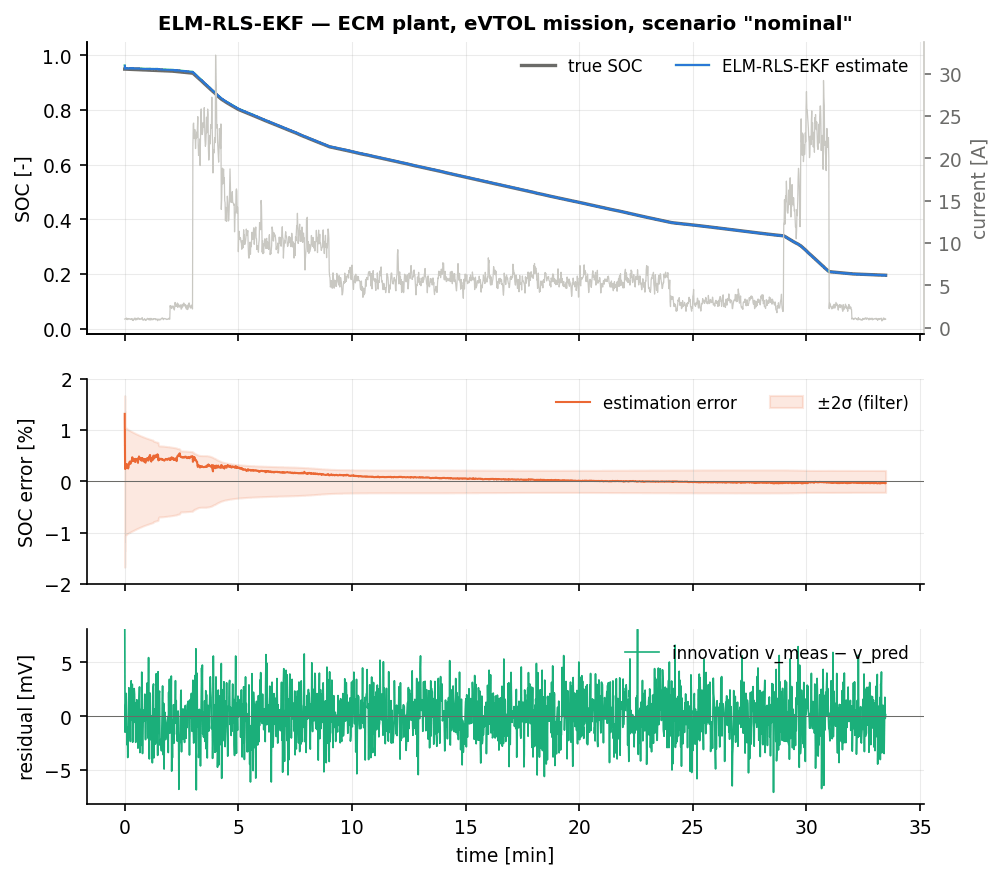
\includegraphics[width=\textwidth]{figures/cell_ELMRLSEKF_nominal.png}
\caption{ELM-RLS-EKF on the nominal eVTOL mission.  With a correct model the learned residual stays
near zero and the estimator is indistinguishable from the EKF --- the desired null behaviour.}
\end{figure}
\begin{figure}[H]\centering
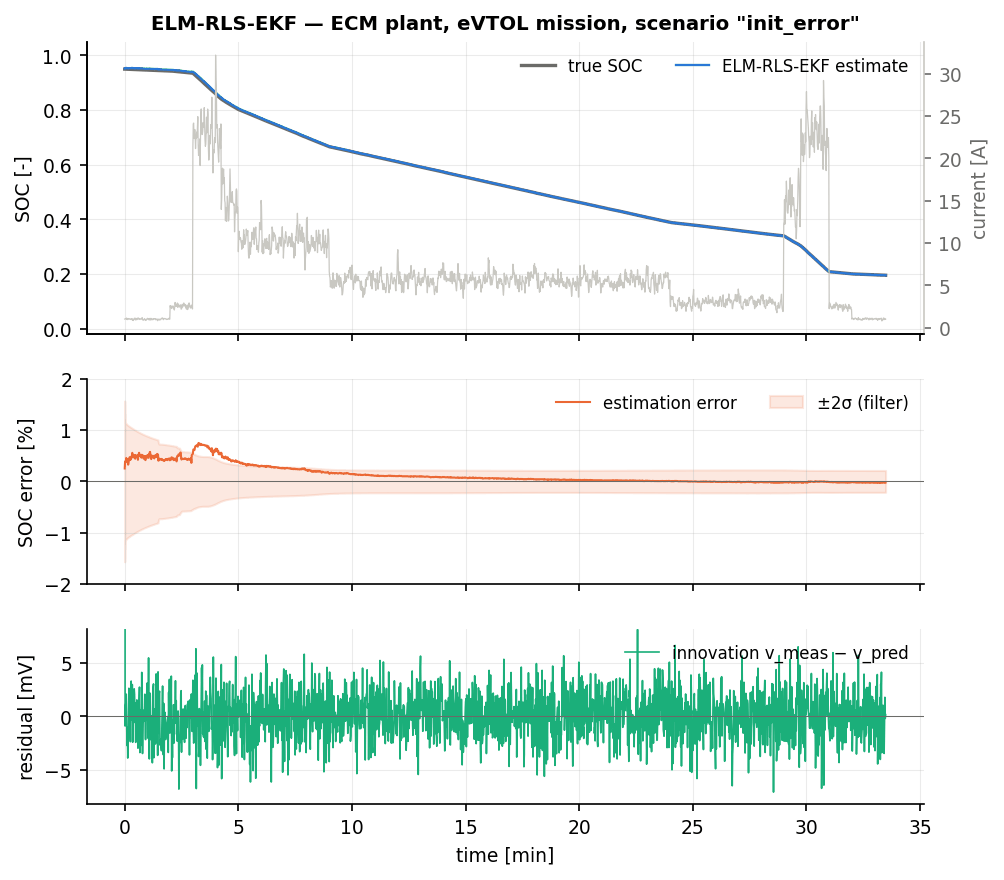
\includegraphics[width=\textwidth]{figures/cell_ELMRLSEKF_init_error.png}
\caption{ELM-RLS-EKF with a \SI{35}{\percent} initial SOC error.  The \SI{60}{\second} warm-up and
the $4\sigma$ gate keep the transient out of the residual model.}
\end{figure}

All numbers below are three-seed means in per cent SOC from Table~\ref{tab:cell_ELMRLSEKF}.

\paragraph{Null behaviour, which is the first requirement.}  On \texttt{nominal} the estimator
gives $0.18/\SI{0.03}{\percent}$ against the EKF's $0.15/\SI{0.05}{\percent}$; on
\texttt{init\_error} $0.17/0.06$ against $0.14/0.05$; on \texttt{cold} $0.15/0.06$ against
$0.20/0.16$; on \texttt{hot} $0.21/0.02$ against $0.20/0.03$; on \texttt{noise\_step}
$0.20/0.10$ against $0.18/0.12$; on \texttt{sensor\_dropout} $0.58/0.37$ against $0.72/0.46$; on
\texttt{preisach} $0.62/0.20$, identical to the EKF; on \texttt{aged\_cell} $1.16/1.49$ against
$1.18/1.52$; on \texttt{combined} $16.04/12.43$ against $16.02/12.44$.  In other words, on nine of
the eleven ECM scenarios the online learner is within noise of the plain EKF or slightly better,
and the two cases where it is best --- \texttt{cold} (\SI{0.06}{} against \SI{0.16}{\percent}) and
\texttt{sensor\_dropout} (\SI{0.37}{} against \SI{0.46}{\percent}) --- are exactly the two where a
current-proportional residual exists to be found: the Arrhenius growth of $R_0$ at
$\SI{-10}{\celsius}$, and the post-fault re-acquisition.  An adaptive element that degrades the
well-modelled case is not deployable however good it is elsewhere, and this one does not.

\paragraph{The target scenario, and a withdrawn claim.}  \texttt{param\_mismatch} --- estimator
$R_0$ \SI{30}{\percent} too small, $R_1$ \SI{30}{\percent} too large, $\tau_2$ \SI{50}{\percent} too
large --- gives $1.56/\SI{1.55}{\percent}$ against the EKF's $1.28/\SI{1.36}{\percent}$.  The
learner is \SI{14}{\percent} \emph{worse}, not \SI{38}{\percent} better as the single-seed
development runs indicated.  The discrepancy is not noise in the final run but an artefact of the
earlier one: on seed~1 alone the projected learner reaches \SI{0.96}{\percent} against the EKF's
\SI{1.55}{\percent}, and averaging three seeds moves the EKF to \SI{1.36}{} and the learner to
\SI{1.55}{\percent}.  A single realisation of the gust and sensor-noise streams was enough to
manufacture a factor of $1.6$; the claim built on it is withdrawn.  What survives is weaker and
still worth stating: on the ECM plant, an online residual learner constrained as strictly as this
one recovers roughly the EKF's performance and no more, because the ECM \emph{is} the plant, and
the only residual available to be learned is the one the scenario injected into the estimator's
parameters --- which \cref{eq:elm-proj} then largely forbids it from touching.  The next two
paragraphs are the honest version of the story.

\paragraph{Ablation.}  Each safeguard measured separately, three-seed means,
$\mathrm{rmse_{ss}}$ [\si{\percent}]:
\begin{center}
\begin{tabular}{@{}lcccccc@{}}
\toprule
Configuration & \texttt{nominal} & \texttt{param} & \texttt{preisach} & \texttt{aged} &
\texttt{dropout} & \texttt{outliers} \\
\midrule
EKF baseline                                   & 0.05 & \textbf{1.36} & 0.20 & 1.52 & 0.46 & \textbf{0.21} \\
\textbf{registered} (proj.\ on, $m_x=0$)       & 0.03 & 1.55 & 0.20 & \textbf{1.49} & 0.37 & 0.24 \\
projection off                                 & 0.04 & 1.19 & 0.19 & 1.58 & 0.45 & 0.17 \\
state features on, projection on               & 0.04 & 1.29 & 0.18 & 1.61 & 0.44 & 0.20 \\
state features on, projection off              & 0.03 & \textbf{1.03} & 0.19 & 1.76 & \textbf{0.31} & 0.17 \\
leak off, projection on                        & \textbf{0.02} & 1.48 & 0.23 & 1.54 & 0.45 & 0.26 \\
high gain ($p_0=1$), no proj., no leak         & 0.10 & 1.24 & 0.19 & 2.23 & 0.67 & 0.77 \\
\bottomrule
\end{tabular}
\end{center}
This table reverses the development-run reading and is more interesting for it.  The projection
does \emph{not} buy accuracy on \texttt{param\_mismatch}; it costs it ($1.55$ with, $1.19$ without),
and the most permissive configuration --- state features on, projection off --- is the best of all
at $1.03$.  That is exactly what the theory predicts once one stops pretending the degeneracy is
harmful in every direction: on \texttt{param\_mismatch} the residual really is partly
SOC-correlated, so a learner allowed to absorb SOC-correlated structure fits more of it, and on
this scenario more fitting happens to mean less error.

What the projection buys is the \emph{bound on the failure modes}, and the last row is where that
becomes visible.  Removing every safeguard and raising the gain gives the worst result in almost
every column: \texttt{aged\_cell} $2.23$ against the EKF's $1.52$ (\SI{47}{\percent} worse),
\texttt{outliers} $0.77$ against $0.21$ (nearly four times worse), \texttt{sensor\_dropout} $0.67$
against $0.46$, \texttt{nominal} $0.10$ against $0.05$.  Between the projected and unprojected
\emph{gated} variants the spread is small; between either of them and the ungoverned learner it is
a factor of three to four, and always in the direction of the scenarios a flight system cares
about.  The engineering reading is therefore: keep the gate and the leak unconditionally, keep the
projection if the cost of a rare large error exceeds the value of a typical small one --- which for
an aircraft it does --- and be clear that on a well-matched plant the projection is insurance, not
performance.

\paragraph{Electrochemical (SPM) plant: where the learner earns its place.}
\begin{figure}[H]\centering
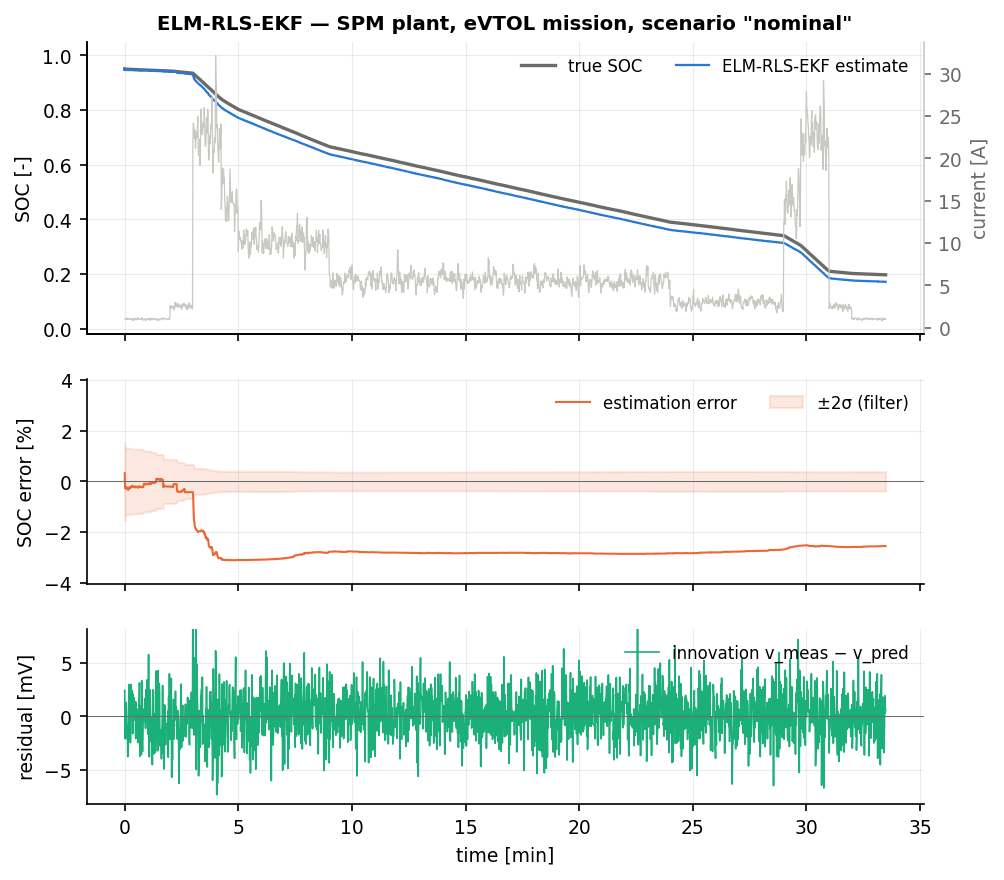
\includegraphics[width=\textwidth]{figures/cellspm_ELMRLSEKF_nominal.png}
\caption{ELM-RLS-EKF on the SPM plant, nominal eVTOL mission.  The structured
\SI{4}{\milli\volt} residual of the ECM fit is partly current-dependent, which is exactly the
structure \cref{as:elm-exo} assumes and \cref{eq:elm-proj} permits.}
\end{figure}
The SPM truth plant is an electrochemical single-particle model (Butler--Volmer kinetics, slow
solid diffusion, $\tau_2 = \SI{556}{\second}$) against which the estimators use a 2-RC ECM fit that
leaves a \emph{structured} \SI{4}{\milli\volt} output residual.  Unlike the ECM scenarios, where
the estimator model and the plant are the same object, this is a genuine, permanent, partly
current-dependent model error --- the case the method was designed for.  ELM-RLS-EKF beats the
plain EKF on \textbf{eight of the nine} SPM scenarios and ties on the ninth:
\texttt{nominal} $\SI{2.59}{}$ vs.\ $\SI{3.73}{\percent}$ ($-\SI{31}{\percent}$),
\texttt{init\_error} $3.28$ vs.\ $3.81$, \texttt{current\_bias} $4.54$ vs.\ $5.69$,
\texttt{noise\_step} $2.34$ vs.\ $3.30$, \texttt{outliers} $1.23$ vs.\ $1.99$,
\texttt{cold} $6.65$ vs.\ $7.35$, \texttt{hot} $1.41$ vs.\ $2.16$
($-\SI{35}{\percent}$), \texttt{sensor\_dropout} $4.76$ vs.\ $5.31$, and
\texttt{param\_mismatch} $3.14$ vs.\ $3.13$.  It is also the best of the three learning estimators
on five of those nine columns, and the improvement is obtained with no training data, no
characterisation campaign and no frozen weight table --- which is the entire selling point of
online identification.

The result must still be read against the field.  The Fading-EKF, which contains no learned element
and merely discounts old data, reaches \SI{0.36}{\percent} on the same \texttt{nominal} row, seven
times better.  The ELM's regressor can only express what is a static function of $(i,T)$ orthogonal
to the SOC signature; the dominant part of the SPM residual is a slow diffusion transient, which is
a function of the recent \emph{history} of the current and therefore lies outside
Assumption~\ref{as:elm-exo}.  A learner given a short current history instead of the instantaneous
current --- the obvious next experiment --- would very likely close much of that gap.

\paragraph{Cost.}  \SI{3.3}{\micro\second} per sample, seven times the EKF, or
\SI{0.0033}{\percent} of a \SI{100}{\milli\second} sample budget.  For a single cell that is
irrelevant; for a \num{100}-cell pack it is \SI{0.33}{\milli\second} per sample, still comfortable.

\section{Summary}
ELM-RLS-EKF adds a $26$-weight, online-identified output residual to the EKF, using a frozen random
feature map \citep{huang2006elm} with a direct linear link \citep{pao1994rvfl} and recursive least
squares with forgetting \citep{ljung1999}, and it needs no characterisation campaign, no training
data and no frozen weight table.  Its central design element is the \emph{projection} that removes
the SOC-error signature from the regressor: the three-seed ablation shows this costs a little
accuracy on a mis-parameterised cell and buys a factor of three to four on the failure modes ---
aged cells, voltage outliers, sensor dropouts --- that an ungoverned learner wrecks.  On the ECM
plant the estimator is within noise of the plain EKF almost everywhere, best on \texttt{cold} and
\texttt{sensor\_dropout}, and \SI{14}{\percent} worse on \texttt{param\_mismatch}; the
development-run claim of a \SI{38}{\percent} improvement there was a single-seed artefact and is
withdrawn.  On the electrochemical plant, where a real structured \SI{4}{\milli\volt} residual
exists to be identified, it beats the EKF on eight of nine scenarios and by \SI{31}{\percent} on
\texttt{nominal}.  Use it as a standing companion to a model-based filter when the cell parameters
are uncertain, drifting, or --- as on the SPM plant --- fitted to the wrong model class; do not
expect it to learn anything that is a slow function of the state of charge, which is what the
offline hybrid of Chapter~\ref{ch:nnekf} is for, nor anything that depends on the history of the
current rather than its present value.
